\documentclass[a4paper]{article}
\usepackage[T1]{fontenc}
\usepackage[utf8]{inputenc}
\usepackage[english]{babel}
\usepackage[hidelinks]{hyperref}
\usepackage{graphicx}
\usepackage{times}
\usepackage{amssymb}
\usepackage{amsmath}
\usepackage{amsthm}
\usepackage{float}
\restylefloat{table}
\usepackage{multicol}
\usepackage{wasysym}
\usepackage[square,sort,comma,numbers]{natbib}
\usepackage{pgfplots}
\pgfplotsset{compat=1.3}
\usepackage{tikz}
\usetikzlibrary{positioning}
\usepackage{fancyvrb}
\usepackage{enumerate}
\fvset{tabsize=3}
\fvset{fontsize=\small}
\newcommand{\code}{\texttt}
\newtheorem{lemma}{Lemma}

\title{\huge{Chromatic Polynomials in Small Space -- Performance in Practice}}

\author{Mats Rydberg\thanks{Master's Thesis student at the Department of Computer Science, Faculty of Engineering (LTH) at Lund University, Lund, Sweden. E-mail: \code{dt08mr7@student.lth.se}. This work was conducted as a part of the authors Master's Thesis project. Supervisor: Thore Husfeldt, prof. in Comp. Science at LTH.}}
\date{\today}

\begin{document}

\maketitle

\begin{abstract}
The \emph{chromatic polynomial} $\chi_G(t)$ of a graph $G$ on $n$ vertices is a univariate polynomial of degree $n$, passing through the points $(q, P(G,q))$ where $P(G,q)$ is the number of $q$-colourings of $G$. In this paper, we present an implementation of an algorithm by Björklund, Husfeldt, Kaski and Koivisto that computes $\chi_G(t)$ in time $O^*(2^n)$ and space $O^*(1.2916^n)$. We compare the performance of two different core libraries to eachother and show our performance against an implementation done by Haggard, Pearce and Royle from 2010. 
We also present the chromatic polynomials for a small Queen graph and a certain graph specified by Hillar and Windfeldt.
\end{abstract}

\newpage

\section{Introduction}

A \emph{proper $q$-colouring} of a graph $G = (V, E)$ is a mapping $\sigma: V \rightarrow [q]$ where $[q] = \{1,2,\ldots,q\}$ such that $\sigma(v) \neq \sigma(w)$ for each $vw \in E$. In other words, $\sigma$ is an assignment of a \emph{colour} to each vertex $v$ such that no two adjacent vertices get the same colour.
The number of ways to $q$-colour $G$ is $P(G,q)$, and the \emph{chromatic polynomial} $\chi_G(t)$ of a graph $G$ passes through each point $(q, P(G,q))$. In other words, it \emph{counts} the number of ways to colour $G$ for any amount of colours.
In particular, the \emph{chromatic number} is the smallest $c$ for which $\chi_G(c) > 0$. The polynomial $\chi_G(t)$ is of high interest in the field of algebraic graph theory, as one of the main graph invariants. Graph colouring is a canonical NP-hard problem, but it also has practical applications for register allocation, scheduling, pattern matching, and in statistical physics, the chromatic polynomial occurs as the zero-temperature limit of the antiferromagnetic Potts model (see for instance \cite{chaitin}, \cite{marx}, and \cite{pottsmodel}).

\subsection{Previous work}
The chromatic polynomial was specified in 1912 by Birkhoff \cite{birkhoff}, who defined it for planar graphs with the intent on proving the Four Colour Theorem. Whitney extended its definition to general graphs in 1932 \cite{whitney}, and Tutte incorporated it into what is now known as the Tutte polynomial.
In 2010, Haggard, Pearce and Royle \cite{haggard} published a program (referred to here as \textbf{HPR}) to compute the Tutte polynomial for graphs using a deletion-contraction algorithm.
The basic idea behind HPR goes back to Zykov~\cite{aazykov}, using cached subgraphs and isomorphism rejection to obtain good performance, and it can easily handle many instances of non-trivial sizes. 
Using the fact that the Tutte polynomial encodes the chromatic polynomial (as well as other graph invariants), HPR is also designed to output $\chi_G(t)$. 
In 2011, Björklund, Husfeldt, Kaski and Koivisto \cite{cov_pack} presented an algorithm to compute the chromatic polynomial in time $O^*(2^n)$ and space $O^*(1.2916^n)$, referred to here as the \textbf{BHKK} algorithm.

\subsection{Results}
In this paper, we present an implementation of the BHKK algorithm and experimental results from running it on selected classes of graphs. In particular, we show that for random graphs with $|V| > 21$, the BHKK algorithm performs consistently better than the HPR algorithm, both in time and space consumption. For practically all nonempty graphs BHKK consumes less memory. Our results also show that in practice, the implementation of polynomial arithmetic is crucial, and has a large impact on overall performance.

Furthermore, we give the chromatic polynomial of a graph, here referred to as Akbari's graph from Akbari, Mirrokni and Sadjad \cite{akbari}, discussed in Hillar and Windfeldt \cite{hillar_windfeldt}, which Maple was unable to compute.
We also give the chromatic polynomial of the queen graph of size $5 \times 5$ (on 25 vertices).

\section{The algorithm}
The algorithm implemented and measured in this paper is described in Björklund \emph{et al} \cite{cov_pack}, and is based on a linear-space Fast Zeta Transform described in the same paper. It is proven to perform in time $O^*(2^n)$ and space $O^*(1.2916^n)$ under certain design parameters. The measured theoretical unit of time is the time it takes to perform an addition or a multiplication of two polynomials of degree $n$. The measured theoretical unit of space is the memory needed to store such a polynomial. In practice, we can not discern this space and time from the space and time used by other parts of needed data structures, but since these dominate, we can assume that the measured space and time usage will converge asymptotically with the theoretical bounds.

Our input is an undirected graph $G$ on $n$ vertices with $m$ edges\footnotemark. The main subroutine counts the number of ways to colour $G$ using $q$ colours. This is done for $q = 0, 1, \ldots n$, yielding $n + 1$ points $(x_i, y_i)$. These are by definition points which the chromatic polynomial $\chi_G(t)$ passes through. $\chi_G(t)$ has exactly degree $n$, and so we have enough information to recover it explicitly (i.e., specifying its coefficients) using interpolation.

\footnotetext{Multiple edges and self-edges are two types of edges that often need special treatment in graph-based algorithms. This is not the case for graph colouring. Any self-edge means the graph is not colourable (a vertex would need to have a different colour from itself), so in this implementation we assume they do not exist. Any multiple edge doesn't affect the problem at all, as we are merely considering the \emph{existence} of an edge between two vertices; if there are more than one that doesn't matter.}

The general idea of the algorithm uses the principle of inclusion-exclusion to count the proper $q$-colourings of $G$ by actually counting the number of ordered partitions of $V$ into $q$ \emph{independent sets}. The low space bound is obtained by splitting $V$ into two disjoint sets $V_1$ and $V_2$ of sizes $n_1$ and $n_2$ respectively, where $n_1 = \lceil n \frac{\log2}{\log3} \rceil$ and $n_2 = n - n_1$, and then run iterations of subsets of $V_1$ and store values dependent on (subsets of) $V_2$ \cite[sec. 5]{cov_pack}. 

The full algorithm is found specified in \cite[p. 9]{cov_pack}. In short, we count the $q$-colourings for each $q \leq n$ independently, and interpolate on the resulting points. When counting colourings, we use an array of polynomials of degree $q$, constructed by analyzing independent subsets. An important aspect is that the main loop executes for subsets of $V_1$, independently from eachother. This allows us to execute all these loop iterations in parallel.

\subsection{Optimizations}\label{opts}
Here are presented some improvements to the algorithm that are either natural, mentioned in \cite{cov_pack}, or invented by the author. This list is by no means exhaustive, nor is every item critical, but the ones we've explored proved to be efficient.

\paragraph{Exploiting $q$}
First, we can consider optimizing on the basis of the value of $q$.
\begin{itemize}
\item For $q = 0$, there are 0 colourings, as no graph can be 0-coloured.
\item For $q = 1$, there are 0 colourings if and only if $|E| > 0$, otherwise there is exactly 1 colouring. This takes $O(n^2)$ time to check.
\item For $q = 2$, it is well-known that the graph can be coloured (or found to be non-colourable) in polynomial time using standard techniques (such as depth-first search).
\end{itemize}

\paragraph{Using $\omega_{min}(G)$}
A more sophisticated type of optimization involves exploiting the clique number $\omega(G)$, which is a lower bound on the chromatic number $\chi(G)$. Knowing that $\omega(G) \geq a$ for some constant $a$ would allow us to omit counting colourings for all $q < a$. If $a = n$, we have the complete graph $K_n$, for which $\chi_G(t)$ is known.

Here we define the \emph{density} of a graph $G$ as $dE = m/\binom{n}{2}$, where $m$ is the number of edges in $G$. This immediately tells us the \emph{smallest possible} $\omega(G)$. Let us call it $\omega_{min}(G)$. In fact, the following holds:

\begin{lemma}\label{lemma1}
The number $\omega_{min}(G)$ is the lower bound of $\omega(G)$, and its value is
\[
\omega_{min}(G) = 
\begin{cases}
	  n - \binom{n}{2} + m & \text{if } m \geq \binom{n}{2} - \lfloor n/2 \rfloor \\
	  \lceil n / 2 \rceil - a & \text{if }  \lfloor n / 2 \rfloor \cdot \lceil n / 2 \rceil < m = \binom{n}{2} - a \lfloor n/2 \rfloor, a \in \mathbb{N}_+ \\
	  2 & \text{if } 0 < m \leq \lfloor n / 2 \rfloor \cdot \lceil n / 2 \rceil \\
	  1 & \text{if } m = 0 \\
\end{cases}
\]
\end{lemma}

\begin{proof}
 Trivially, $w(N_n) = 1$. This proves the lower-most bound.
 
 Next, consider the complete bipartite graph $K_{\alpha,\beta}$ on $n$ vertices; it is the graph with the most edges that has clique number 2. It is well-known that it has $\alpha \beta$ edges. To maximize this product, we make a half-half partition, setting $\alpha = \lfloor n / 2 \rfloor$ and $\beta = \lceil n / 2 \rceil$, giving $\alpha \beta = \lfloor n / 2 \rfloor \lceil n / 2 \rceil$. The point made is that there is no way of assigning more edges than this without yielding a higher clique number.
 
 Third, consider the complete graph $K_n$, with $w(K_n) = n$. Deleting an edge $vw$ will clearly reduce the clique number. Consider the subgraph $K \setminus \{v\}$; it has clique number $n - 1$. Removing an edge $uu', u \neq w, u' \neq w$ will lower clique number again by 1. This process may be repeated $\lfloor n / 2 \rfloor$ times. The resulting graph has $\binom{n}{2} - \lfloor n/2 \rfloor$ edges and clique number $n - \lfloor n/2 \rfloor$. This, together with the fact that removing one edge can lower clique number by maximum one, proves the uppermost bound. 
\end{proof}

For the final case, for which we do not provide a full proof, we observe that $\binom{n}{2} - \lfloor n/2 \rfloor - \lfloor n / 2 \rfloor \cdot \lceil n / 2 \rceil$ is a multiple of $\lfloor n/2 \rfloor$ (this is the variable $a$ in the lemma). It can be shown that this corresponds to the requirement of removing $\lfloor n/2 \rfloor$ edges to reduce clique number by one.

As we can see from Lemma~\ref{lemma1}, only graphs with $m > \lfloor n / 2 \rfloor \cdot \lceil n / 2 \rceil$ provides $\omega_{min}(G) > 2$ and for $q \leq 2$ we already have good optimizations. So how dense is a graph where this bound on $m$ holds? Let us specify the threshold density $T_{dE}(n)$ as

\[
T_{dE}(n) = 2\frac{\lfloor n / 2 \rfloor \cdot \lceil n / 2 \rceil}{n(n-1)} =
\begin{cases}
	  \frac{1}{2}n(n-1)^{-1} & \text{if } n \text{ even}\\
	  \frac{1}{2}(n+1)n^{-1} = T_{dE}(n+1) & \text{if } n \text{ odd}\\
\end{cases}
\]

In conclusion, any graph with $dE > T_{dE}(n)$ can omit the computation of the number of $q$-colourings when $q \leq w_{min}(G)$. It also follows that as $n \rightarrow \infty$ we will have $T_{dE}(n) \rightarrow \frac{1}{2}$. The following plot shows how fast we converge for graphs of sizes relevant for this paper.

\begin{center}
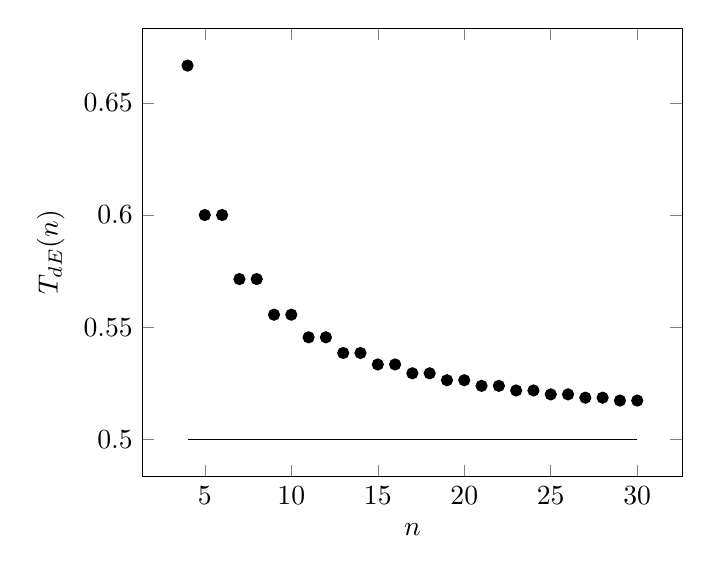
\begin{tikzpicture}
\begin{axis}[
xlabel=$n$,
ylabel=$T_{dE}(n)$]
\addplot[black, only marks, mark=*, samples=14, domain=4:30] {x/(2*(x-1))};
\addplot[black, only marks, mark=*, samples=13, domain=5:29] {(x+1)/(2*x)};
\addplot[black, samples=10, domain=4:30] {1/2};
\end{axis}
\end{tikzpicture}
\end{center}
For larger graphs, we have a smaller $T_{dE}(n)$, which gives us a higher probability to be able to optimize, and it is also for larger graphs that we are most interested in optimizing techniques. For a graph with $n=23$ and $dE = 75$, we would be able to skip evaluating $q\leq7$, which yields a decrease in execution time by about 15\%\footnotemark.

\footnotetext{This number is based on experimental results presented below.}

\paragraph{Parallelization 1} Potentially, we could parallelize the algorithm using $2^{|V_1|} = O^*(1.5486^n)$ CPUs. This would yield significant time improvements in theory, reducing the asymptotic time bound to about $O^*(1.5486^n)$. Using a different partition of $V$ with $n_1 = n_2$, we would achieve space and time bounds of $O^*(2^{n/2})$ on as many CPUs \cite{cov_pack}.

\paragraph{Parallelization 2} Typically, we will only have access to a constant number of CPUs in practice, allowing each of them to not execute one loop iteration but a range of iterations for a range of subsets. This allows for heuristics on how to select such ranges so that the overall time bound (set by the range of subsets that include the \emph{most} independent subsets) is minimal. The currently used heuristic is to simply take the subsets in inorder. As presented below, we can expect to reduce the time consumption of the program by a factor of around 6.

\paragraph{Degree pruning} When multiplying and exponentiating our polynomials, we increase their degree, potentially as large as $qn$ (we exponentiate with $q$). But since we never do any divisions, and never care about coefficients for terms of degree $> n$, we can simply discard these terms, keeping degrees $\leq n$.

\section{Algorithm performance parameters}
The algorithm has some perks that make it perform better or worse for different input. In this section we aim to explore a few of these characteristics.

\subsection{Sparse and dense graphs}\label{sparsedense}
The algorithm in itself is designed in a way that allow for a smaller degree of complexity for \emph{dense} graphs. This is in contrast to many previously studied algorithms for graph colouring problems. And this is not only for very dense graphs, but the performance of the algorithm is in fact a function that is directly related to graph density, and consistently performs better for every additional edge to a graph. This is a direct consequence of the content of the polynomial arrays, which contain non-zero for each \emph{independent} subset considered (see \cite[p. 9, steps 2b and 2c]{cov_pack}). As graph density increases, fewer subsets of the vertex set will be independent, and more polynomials will be equal to zero. This has a direct effect in reducing some additions and assignments, but more importantly has side effects in all subsequent steps, as arithmetic with zero-operands is (much) faster.

\section{Experimental results}
This section presents selected results in four parts. First, we show the metrics for the best implementation currently available, and discuss how it relates to the theory described above. Second, we compare it to some of the other implementations, to visualize the impact of some development choices. Most importantly, we make a comparison between which library for polynomial arithmetic was used. Thirdly, we compare our results to the Haggard-Pearce-Royle implementation.
We end by providing the chromatic polynomials for two small Queen graphs and a graph discussed by Hillar and Windfeldt in \cite{hillar_windfeldt}. 

For the first two parts, the tests are performed on randomized graphs, generated for some values of $n$ and $dE$ using a tool developed by the author. The process is basically to fill an array $A$ of size $\frac{1}{2}n(n-1)$ with $m$ ones and rest zeroes, shuffle $A$ using Fisher-Yates shuffle and then add the edge $v_iv_{i+1}$ to the graph if $A[i] = 1$.

\subsection{Measurements}
All tests are performed on the same machine, with the following specifications.

\begin{center}
\begin{tabular}{l|l}
CPU (cores, threads) & Intel i7-3930K 3.2GHz (6, 12) \\ 
OS & GNU/Linux 3.8.13.4-desktop-1.mga3 (Mageia 3) x86\_64 \\ 
Memory & 16GB DDR3 1333Mhz \\ 
Compiler & GCC 4.7.2 (g++) \\ 
\end{tabular}
\end{center}

For all time and memory measurements, the GNU \code{time} 1.7 program is used (see the Linux man pages \cite{time}). The user time, elapsed time (real time) and peak resident set size are the data points recovered as measurements. These measurements are taken by running the specified program on a number
\footnote{Usually, this is 50 or 100. Smaller for larger graphs because of time restrictions.} 
of graphs of equal size and the average values are the ones presented.

\subsection{\code{bhkk-pari-0.3}}
The most powerful implementation is \code{bhkk-pari-0.3}. It implements these optimizations: $q = \{0, 1\}$, $w_{min}(G)$, parallelization 2, degree pruning. We show here its time and memory consumption in relation to both $n$ and $m$.

\begin{center}
\begin{tabular}{rl}
\begin{tikzpicture}
\begin{semilogyaxis}[title={Random graphs of fixed density},
legend pos=north west,baseline,trim axis left,small,
xlabel=Number of vertices $n$,
ylabel=Average real time (ms)]
\addplot[red,mark=triangle*] table[x=n,y=rt] {tables/bhkk-pari-0.3_1};
\addplot[blue,mark=asterisk] table[x=n,y=rt] {tables/bhkk-pari-0.3_2};
\legend{$dE = 40$, $dE = 75$, $f_t$}
\end{semilogyaxis}
\end{tikzpicture}
&
\begin{tikzpicture}
\begin{axis}[title={Random graphs of fixed density},
legend pos=north west,baseline,trim axis right,small,
yticklabel pos=right, ylabel style={align=right},
xlabel=Number of vertices $n$,
ylabel=Average peak resident set size (kB)]
\addplot[red,mark=triangle*] table[x=n,y=rss] {tables/bhkk-pari-0.3_1};
\addplot[blue,mark=asterisk] table[x=n,y=rss] {tables/bhkk-pari-0.3_2};
\legend{$dE = 40$, $dE = 75$, $f_m$}
\end{axis}
\end{tikzpicture}
\\
\begin{tikzpicture}
\begin{axis}[title={Random graphs, $n = 19$},
legend pos=north west,baseline,trim axis left,small,
xlabel=Number of edges $m$,
ylabel=Average real time (ms)]
\addplot[red,mark=triangle*] table[x expr=\thisrow{dE}*1.71,y=rt] {tables/bhkk-pari-0.3_3};
\end{axis}
\end{tikzpicture}
&
\begin{tikzpicture}
\begin{axis}[title={Random graphs, $n = 19$},
legend pos=north west,baseline,trim axis right,small,
yticklabel pos=right, ylabel style={align=right},
xlabel=Number of edges $m$,
ylabel=Average peak resident set size (kB)]
\addplot[red,mark=triangle*] table[x expr=\thisrow{dE}*1.71,y=rss] {tables/bhkk-pari-0.3_3};
\end{axis}
\end{tikzpicture}
\\
\end{tabular}
\end{center}

\subsubsection{Power of parallelization}
On the test machine, the actual parallelization width is 12. But using some waiting threads to take over when the fastest threads have terminated seems to be a smarter approach. Actually, we can show that doing so will lower our time requirements by a few percent, but it comes at a very large cost in memory.
\begin{center}
\begin{tabular}{rl}
\begin{tikzpicture}
\begin{semilogyaxis}[title={Random graphs, $dE = 75$},
legend pos=north west,baseline,trim axis left,small,
xlabel=Number of vertices $n$,
ylabel=Average real time (ms)]
\addplot[black,mark=+] table[x=n,y=rt] {tables/bhkk-pari-0.1_2};
\addplot[blue,mark=asterisk] table[x=n,y=rt] {tables/bhkk-pari-0.2_2_12};
\addplot[red,mark=triangle*] table[x=n,y=rt] {tables/bhkk-pari-0.3_1};
\legend{Single thread, $t = 12$, $t = 45$}
\end{semilogyaxis}
\end{tikzpicture}
&
\begin{tikzpicture}
\begin{axis}[title={Random graphs, $dE = 75$},
legend pos=north west,baseline,trim axis right,small,
yticklabel pos=right, ylabel style={align=right},
xlabel=Number of vertices $n$,
ylabel=Average peak resident set size (kB)]
\addplot[black,mark=+] table[x=n,y=rss] {tables/bhkk-pari-0.1_2};
\addplot[blue,mark=asterisk] table[x=n,y=rss] {tables/bhkk-pari-0.2_2_12};
\addplot[red,mark=triangle*] table[x=n,y=rss] {tables/bhkk-pari-0.3_1};
\legend{Single thread, $t = 12$, $t = 45$}
\end{axis}
\end{tikzpicture}
\\
\end{tabular}
\end{center}
\begin{multicols}{2}
As mentioned above, parallelization (of width 12) allows us to terminate about six times faster. Here we plot the parallelization factor $p$ as the quota of the non-parallelized \code{bhkk-pari-0.1} and the fastest implementation \code{bhkk-pari-0.3}.

\columnbreak

\begin{tikzpicture}
\begin{axis}[title={Random dense graphs},
legend pos=north west,baseline,trim axis left,width = 180,height = 80,
ytick={6,7},ymin=5,ymax=7.5,
xtick={14,15,16,17,18,19,20,21,22,23},
xlabel=Number of vertices $n$,
ylabel=$p$]
\addplot[red,mark=*] table[x=n,y expr=\thisrow{0.1} / \thisrow{0.3-45}] {tables/bhkk-pari-0.x_rtimes};
\end{axis}
\end{tikzpicture} 
\end{multicols}


\subsubsection{Polynomial arithmetic library performance}
The most common operation in the algorithm is multiplying two polynomials. Thus the implementation of that operation is critical to performance. In this paper, we omit a more detailed description of the implementation techniques used for the BHKK algorithm, but two reference implementations were made, one linked with the PARI library \cite{pari}, and one with the NTL library \cite{ntl}. To provide a little insight in how important the actual implementation of polynomial arithmetic is, we also show a comparison of the implementation linked with PARI and the one linked with NTL.

\begin{center}
\begin{tabular}{rl}
\begin{tikzpicture}
\begin{semilogyaxis}[title={Random dense graphs},
legend pos=north west,baseline,trim axis left,small,
xlabel=Number of vertices $n$,
ylabel=Average real time (ms)]
\addplot[red,mark=triangle*] table[x=n,y=rt] {tables/bhkk-pari-0.3_2};
\addplot[blue,mark=asterisk] table[x=n,y=rt] {tables/bhkk-ntl-0.3_2};
\legend{PARI, NTL}
\end{semilogyaxis}
\end{tikzpicture}
&
\begin{tikzpicture}
\begin{axis}[title={Random dense graphs},
legend pos=north west,baseline,trim axis right,small,
yticklabel pos=right, ylabel style={align=right},
xlabel=Number of vertices $n$,
ylabel=Average peak resident set size (kB)]
\addplot[red,mark=triangle*] table[x=n,y=rss] {tables/bhkk-pari-0.3_2};
\addplot[blue,mark=asterisk] table[x=n,y=rss] {tables/bhkk-ntl-0.3_2};
\legend{PARI, NTL}
\end{axis}
\end{tikzpicture}
\\
\end{tabular}
\end{center}
As is made clear, NTL is too slow to compete. This of course tempts the question whether there are even faster libraries to use.

\subsection{Relation to other work}
As comparison throughout the development process, we have consistently used HPR. Initially to make sure that the output were the same given same input (and hence, since HPR is a published tool by renowned authors, correct), and eventually, to ``race''. From performance tests that were made, HPR seems to do better if the input has ``some kind of structure'', rather than being ``random''. This is manifested by it performing considerably well on any ``famous'' graph (which usually is famous because such graphs appeal to some ``human sense'' of pattern-recognition). But in the case of graphs generated according to the randomized process mentioned here, HPR does not scale as well as BHKK, and has a ``weak spot'' for graphs of density around 75 \cite{haggard}. More pressingly, HPR does not give good worst-case performance. Our measurements show a large ($> 95\%$) variance\footnotemark in performance on different graphs of equal size. This is not the case with BHKK, which has near-deterministic ($< 15\%$ variance) computation time from given size of input.

\footnotetext{With variance, we mean the number $1 - m/M$, where $M$ is the maximum measured value and $m$ the minimum.}

The main improvement of BHKK is of course the memory consumption. HPR relies on the use of a cache for recognition of isomorphic graphs in order to perform well. In (most of) these test runs we've allowed HPR to use a lot of cache, about 10GB. This is because we wish to show that BHKK can run faster even when HPR is not directly limited by its cache size.
\begin{center}
\begin{tabular}{rl}
\begin{tikzpicture}
\begin{semilogyaxis}[title={Random graphs, $dE = 40$},
legend pos=north west,baseline,trim axis left,small,
xlabel=Number of vertices $n$,
ylabel=Average real time (ms)]
\addplot[blue,mark=asterisk] table[x=n,y=rt] {tables/hpr_1};
\addplot[red,mark=triangle*] table[x=n,y=rt] {../output/javatests/comp_tutte1};
\legend{HPR, BHKK}
\end{semilogyaxis}
\end{tikzpicture}
&
\begin{tikzpicture}
\begin{semilogyaxis}[title={Random graphs, $dE = 40$},
legend pos=north west,baseline,trim axis right,small,
yticklabel pos=right, ylabel style={align=right},
xlabel=Number of vertices $n$,
ylabel=Average peak resident set size (kB)]
\addplot[blue,mark=asterisk] table[x=n,y=rss] {tables/hpr_1};
\addplot[red,mark=triangle*] table[x=n,y=rss] {../output/javatests/comp_tutte1};
\legend{HPR, BHKK}
\end{semilogyaxis}
\end{tikzpicture}
\end{tabular}

\begin{tabular}{rl}
\begin{tikzpicture}
\begin{semilogyaxis}[title={Random graphs, $n = 21$},
legend pos=south west,baseline,trim axis left,small,
xlabel=Number of edges $m$,
ylabel=Average real time (ms)]
\addplot[blue,mark=asterisk] table[x expr=\thisrow{dE} * 2.1,y=rt] {tables/hpr_2};
\addplot[red,mark=triangle*] table[x expr=\thisrow{dE} * 2.1,y=rt] {../output/javatests/comp_tutte2};
\legend{HPR, BHKK}
\end{semilogyaxis}
\end{tikzpicture}
&
\begin{tikzpicture}
\begin{semilogyaxis}[title={Random graphs, $n = 21$},
legend pos=north west,baseline,trim axis right,small,
yticklabel pos=right, ylabel style={align=right},
xlabel=Number of edges $m$,
ylabel=Average peak resident set size (kB)]
\addplot[blue,mark=asterisk] table[x expr=\thisrow{dE} * 2.1,y=rss] {tables/hpr_2};
\addplot[red,mark=triangle*] table[x expr=\thisrow{dE} * 2.1,y=rss] {../output/javatests/comp_tutte2};
\legend{HPR, BHKK}
\end{semilogyaxis}
\end{tikzpicture}
\\
\end{tabular}
\end{center}
These results are somewhat in contrast to those presented in \cite{haggard}. The data here suggests that the ''weak spot'' in terms of density would be around $50\%$, whereas \cite{haggard} suggests ''weak spot'' around $75\%$. It's made clear however, that BHKK shows better asymptotic behaviour, and that the space improvements are significant, also in practice. Note that the first test (upper graphs) were performed on a sparse graph, meaning BHKK is not working under optimal conditions.

\begin{table}[H]\centering
\begin{tabular}{|c|c|c|c|} \hline
  & CPU time (s) & Real time (s) & Peak resident set size (kB) \\ \hline
  $n = 25$, $dE = 75$ & & & \\ \hline
  \code{bhkk-pari-0.2} & 9,492 & 941 & $1.46 \cdot 10^{5}$ \\ \hline
  HPR & - & > 260,000 & - \\ \hline
  $n = 30$, $dE = 75$ &  &  &  \\ \hline
  \code{bhkk-pari-0.2} & 556,895 & 53,834 & $7.41 \cdot 10^{5}$ \\ \hline
  HPR & > 94,000 & > 95,000 & $4.11 \cdot 10^{7}$ \\ \hline
\end{tabular}
\caption{Larger instances. Results are based on a single run on one graph. HPR did not terminate within the times specified here. \code{bhkk-pari-0.2} implements $q = \{0, 1\}$, parallelization 2 and degree pruning.}
\end{table}

\section{Some chromatic polynomials}
Here we provide the actual chromatic polynomials of a few famous graphs, together with data on how expensive these polynomials were to compute.

% (En sak: Skriv något i stil med “The basic idea [of HPR] idea goes back to the deletion-contraction algorithm of Zykov, with cached subgraphs and isomorphism rejection.” 

% Senare, när du nämnar Maple, “which is a naïve implementation of Zykov’s deletion-contraction recurrence”). Jag tror Skiena har beskrivit Maple-implementationen någonstans i en tidigare bok. Men ta med referens til Zykov.

\subsection{Akbari's graph}
Hillar and Windfeldt discussed characterizations of \emph{uniquely} colourable graphs in \cite{hillar_windfeldt}. That is, a graph $G$ with $\chi_G(\chi(G)) = \chi(G)!$, or in other words that there exists only one optimal colouring, unique up to interchangability of the colours. Hillar and Windfeldt makes an attempt to verify their results by determining the chromatic polynomials of two graphs known to be uniquely 3-colourable, in order to test whether $\chi_G(3) = 3!$ for them. However, they were unable to determine the chromatic polynomial of the larger graph (on 24 vertices), Akbari's graph, seen here in figure~\ref{akbaris}, using Maple, as it uses a naive implementation of Zykov's~\cite{aazykov} deletion-contraction recurrence. Using BHKK, we successfully determined $\chi_{Akbari}(t)$:
\begin{equation*}
\begin{split}
\chi_{Akbari}(t) & =  t^{24} - 45t^{23} + 990t^{22} -14174t^{21} + 148267t^{20} - 1205738t^{19} \\ & \quad
+ 7917774t^{18} - 43042984t^{17} + 197006250t^{16} - 767939707t^{15} \\ & \quad 
+ 2568812231t^{14}  - 7407069283t^{13} 
+ 18445193022t^{12} \\ & \quad
- 39646852659t^{11} + 73339511467t^{10} - 116102230203t^9 \\ & \quad
+ 155931129928t^8 - 175431211152t^7 + 162362866382t^6 \\ & \quad - 120414350156t^5 
+ 68794778568t^4 - 28408042814t^3 \\ & \quad + 7537920709t^2 - 963326674t
\end{split}
\end{equation*}
and in particular, $\chi_G(3) = 3!$, as expected. This took $1445$ seconds to compute, using our fastest implementation. HPR however terminated even faster, which was to be expected.

\begin{figure}
\centering
 \begin {tikzpicture}[semithick, inner sep = 1,trim left = -70,
b/.style ={ circle ,draw, text=white, minimum width = 6 mm, fill = black!100},
g/.style ={ circle ,draw, text=blue, minimum width = 6 mm, fill = black!50},
w/.style ={ circle ,draw, text=black, minimum width = 6 mm, fill = white!0}]
\node[g] (1) at (-2,-2) {$1$};
\node[b] (2) at (-2,3) {$2$}
  edge [-] (1);
\node[w] (3) at (3,3) {$3$}
  edge [-] (2);
\node[w] (4) at (3,-2) {$4$}
  edge [-] (1);
\node[g] (5) at (-1,0) {$5$};
\node[b] (6) at (-1,1) {$6$}
  edge [-,bend right =10] (1)
  edge [-] (5);
\node[w] (7) at (0,2) {$7$}
  edge [-] (2)
  edge [-] (6);
\node[g] (8) at (1,2) {$8$}
  edge [-] (7);
\node[b] (9) at (2,1) {$9$}
  edge [-, bend left = 10] (4)
  edge [-] (5)
  edge [-] (8);
\node[g] (10) at (2,0) {$10$}
  edge [-, bend right = 10] (3)
  edge [-] (6);
\node[b] (11) at (1,-1) {$11$}
  edge [-] (4)
  edge [-] (7)
  edge [-] (10);
\node[w] (12) at (0,-1) {$12$}
  edge [-] (1)
  edge [-] (5)
  edge [-] (8)
  edge [-] (11);
\node[b] (13) at (10,-2) {$13$};
\node[w] (14) at (5,-2) {$14$}
  edge [-, bend left = 80] (2)
  edge [-] (10)
  edge [-] (13);
\node[g] (15) at (5,3) {$15$}
  edge [-, bend right = 35] (7)
  edge [-] (14);
\node[g] (16) at (10,3) {$16$}
  edge [-] (13);
\node[w] (17) at (8,-1) {$17$};
\node[g] (18) at (7,-1) {$18$}
  edge [-, bend left = 25] (3)
  edge [-, bend right = 10] (13)
  edge [-] (17);
\node[b] (19) at (6,0) {$19$}
  edge [-] (14)
  edge [-] (18);
\node[w] (20) at (6,1) {$20$}
  edge [-] (19);
\node[b] (21) at (7,2) {$21$}
  edge [-, bend left=10] (16)
  edge [-] (17)
  edge [-] (20);
\node[b] (22) at (8,2) {$22$}
  edge [-, bend right = 45] (10)
  edge [-, bend right = 20] (15)
  edge [-] (18)
  edge [-] (21);
\node[w] (23) at (9,1) {$23$}
  edge [-] (16)
  edge [-] (19)
  edge [-] (22);
\node[g] (24) at (9,0) {$24$}
  edge [-] (13)
  edge [-] (17)
  edge [-] (20)
  edge [-] (23);
  
  \pgfresetboundingbox
  \draw (-2,-3)  (10,3);
\end{tikzpicture}
 \caption{Akbari's graph, coloured in its unique 3-colouring with white, gray and black as colours. Figure copied from figure~2 in \cite{hillar_windfeldt}.}
 \label{akbaris}
\end{figure}

\subsection{Queen graph}

The $n \times n$ \emph{Queen graph} is a graph laid out like a chess board with $n$ squares per side. Each square is a vertex and it has edges to all squares in its column, in its row and in its diagonals. In other words, to each square to which a queen could move, if placed on said square. Here we provide the chromatic polynomial of the $5 \times 5$ Queen graph $Q_5$, on 25 vertices.

\begin{equation*}
\begin{split}
\chi_{Q_5}(t) & = t^{25} -160t^{24} + 12400t^{23} -619000t^{22} + 22326412t^{21} -618664244t^{20} \\ & \quad 
+ 13671395276t^{19} -246865059671t^{18} + 3702615662191t^{17} \\ & \quad
-46639724773840t^{16} + 496954920474842t^{15}  -4497756322484864t^{14} \\ & \quad 
+ 34633593670260330t^{13} -226742890673713726t^{12} \\ & \quad 
+ 1258486280066672806t^{11} -5890734492089539317t^{10} \\ & \quad 
+ 23071456910844580538t^9 -74774310771536397886t^8 \\ & \quad  
+ 197510077615138465516t^7 -416375608854898733286t^6  \\ & \quad 
+ 680208675481930270860t^5 -824635131668099993614t^4 \\ & \quad 
+ 692768396747228503860t^3 -356298290543726707632t^2  \\ & \quad 
+ 83353136564448062208t
\end{split}
\end{equation*}

\begin{table}[H]\centering
\begin{tabular}{|c|c|c|c|} \hline
  Algorithm & Real time (s) & Peak resident set size (kB) \\ \hline
  BHKK & 1453 & 199216 \\ \hline
  HPR & 2727 & 41094832 \\ \hline
\end{tabular}
\caption{Time and memory measurements on computing the chromatic polynomial of $Q_5$.}
\end{table}

\bibliographystyle{12page}

\bibliography{bhkk_paper}

\end{document}